%%%%%%%%%%%%%%%%%%%%%%%%%%%%%%%%%
\section{Production and Quality Assurance}
\label{sec:dp-tpcelec-production}

\fixme{This was repetitive. I think we just need a sentence here about how some items will be purchased commercially, DUNE will produce and test other items... then move straight into the subsections}
%We envision splitting production of the electronics system components among several sites in France and Japan. The delivered components will be divided between institutions in France, Japan, and the USA, where they will be tested and calibrated (analog \dword{fe} cards and \dwords{amc}). Each card test site will be equipped to do \dword{qc} and \dword{qa} checks as well as perform calibration of analog and digital cards. Based on the experience with the production of \dword{cro} readout electronics for \dword{pddp}, Figure~\ref{fig:dp-tpcelec-qc-chain} schematically illustrates the necessary equipment and set-up for these tasks.

%A \dword{utca} crate equipped with \dword{mch} and \dword{wrmch} will host \dwords{amc} to be tested and calibrated. Triggering follows the same scheme as in \dword{pddp} relying on the distribution of timestamped trigger packets over the \dword{wr} network to \dwords{amc}. The triggers are generated by a high precision pulse generator synchronously with the calibration pulse signals sent to the analog or digital electronics. For \dword{cro} the electronics, a dedicated calibration cards has been developed to inject via a precision capacitor a known amount of charge into individual \dword{asic} channels to verify their functionality and calibrate the gain of the amplifiers. The channels selection is automatically performed via a multiplexer. The calibration of \dword{adc} buffer of the \dword{cro} \dwords{amc} is accomplished by injecting a known pulse into input stage and measuring the resultant pulse height after the digitization. 

%The following sub-sections provide additional details on \dword{qc} and \dword{qa} for specific sub-systems. Some calibration results from \dword{pddp} card production are also included.
%\fixme{A brief introductory statement would clarify the section logic for readers.}


%%%%%%%%%%%%%%%%%%%%%%%%%%%%%%%%%
\subsection{Cryogenic Analog FE Electronics}
\label{ssec:dp-tpcelec-prod-cryofe}

%The production of the cryogenic \dwords{asic} and analog \dword{fe} cards takes place at several sites in France and Japan. The delivered cards are divided among five institutions in France (IPNL), Japan (KEK, NITKC, IU), and USA (SMU), where they are tested for various performance parameters such as noise levels, dead channels, hot channels, and gain and its uniformity across channels, at both room and operating cold temperature. Each testing site will be contain a copy of system shown in Figure~\ref{fig:dp-tpcelec-qc-chain} and an appropriate and common database will be developed and populated with test results. 
The production of the cryogenic \dwords{asic} and analog \dword{fe} cards takes place at several sites in France and Japan. Five institutions (IPNL in France; KEK, NITKC, and IU in Japan, and SMU in the USA) will share testing responsibilities. Cards will be shipped to these testing sites where collaborators will check performance parameters such as noise levels, dead channels, hot channels, and gain and its uniformity across channels, at both room and operating cold temperature. Based on the \dword{pddp} experience, each testing site will have a system like that shown in Figure~\ref{fig:dp-tpcelec-qc-chain}. %and an appropriate and 
A common database will be developed and populated with test results. 

\begin{dunefigure}[Overview of the configuration for quality control and calibration of \dword{cro} electronics system]{fig:dp-tpcelec-qc-chain}
{Overview of the configuration for quality control and calibration of \dword{cro} electronics system.}
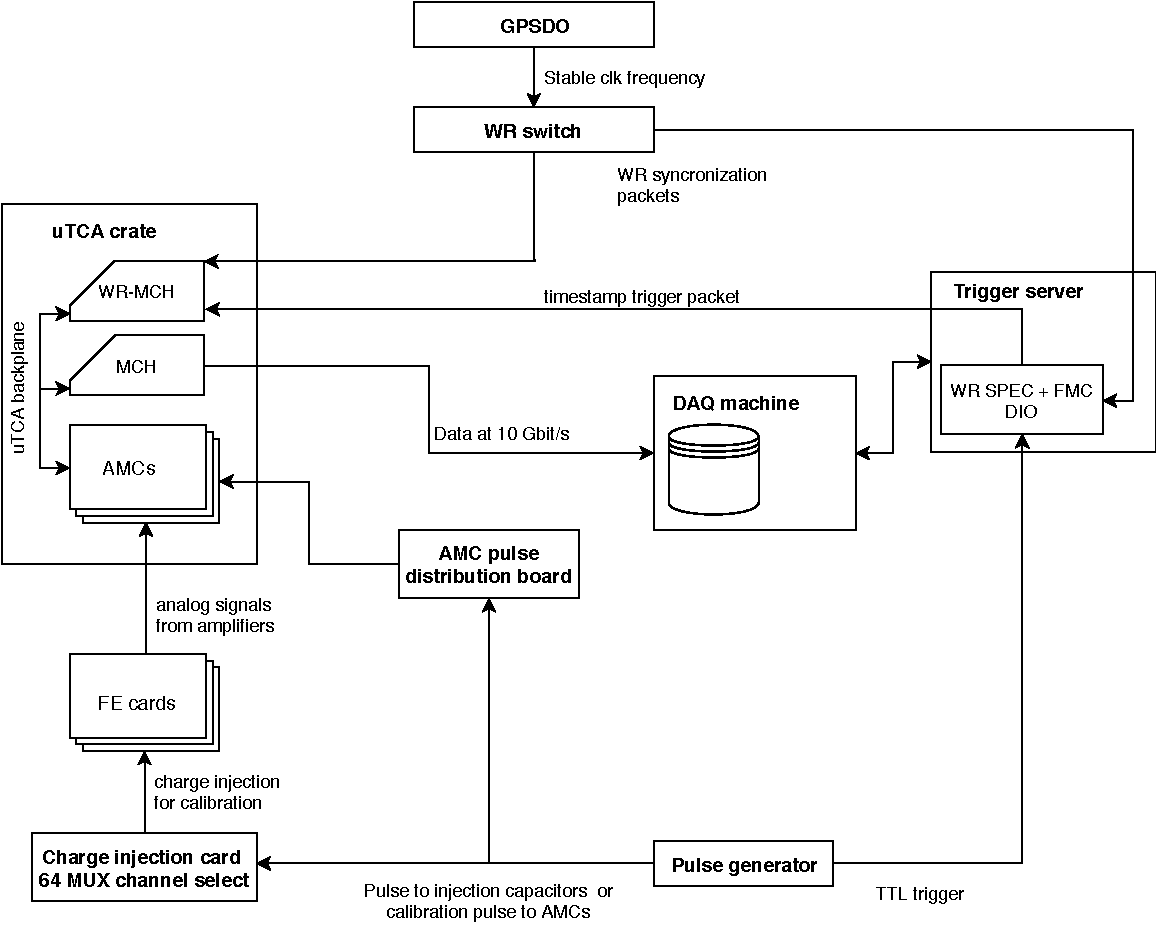
\includegraphics[width=0.8\textwidth]{dp-tpcelec-qc-chain}
\end{dunefigure}
\fixme{this figure could use a bit more explanation} 

\begin{dunefigure}[Channel-to-channel gain uniformity measured on \dword{fe} cards produced for \dword{pddp}]{fig:dp-tpcelec-fec-calib}
{Channel-to-channel gain uniformity measured on \dword{fe} cards produced for \dword{pddp}. The plot on the left illustrates the gain (in units of pulse integral per unit of injected charge) as a function channel number for all the tested cards, while that on the right shows the overall distribution of the gain values fitted to the Gaussian function.}
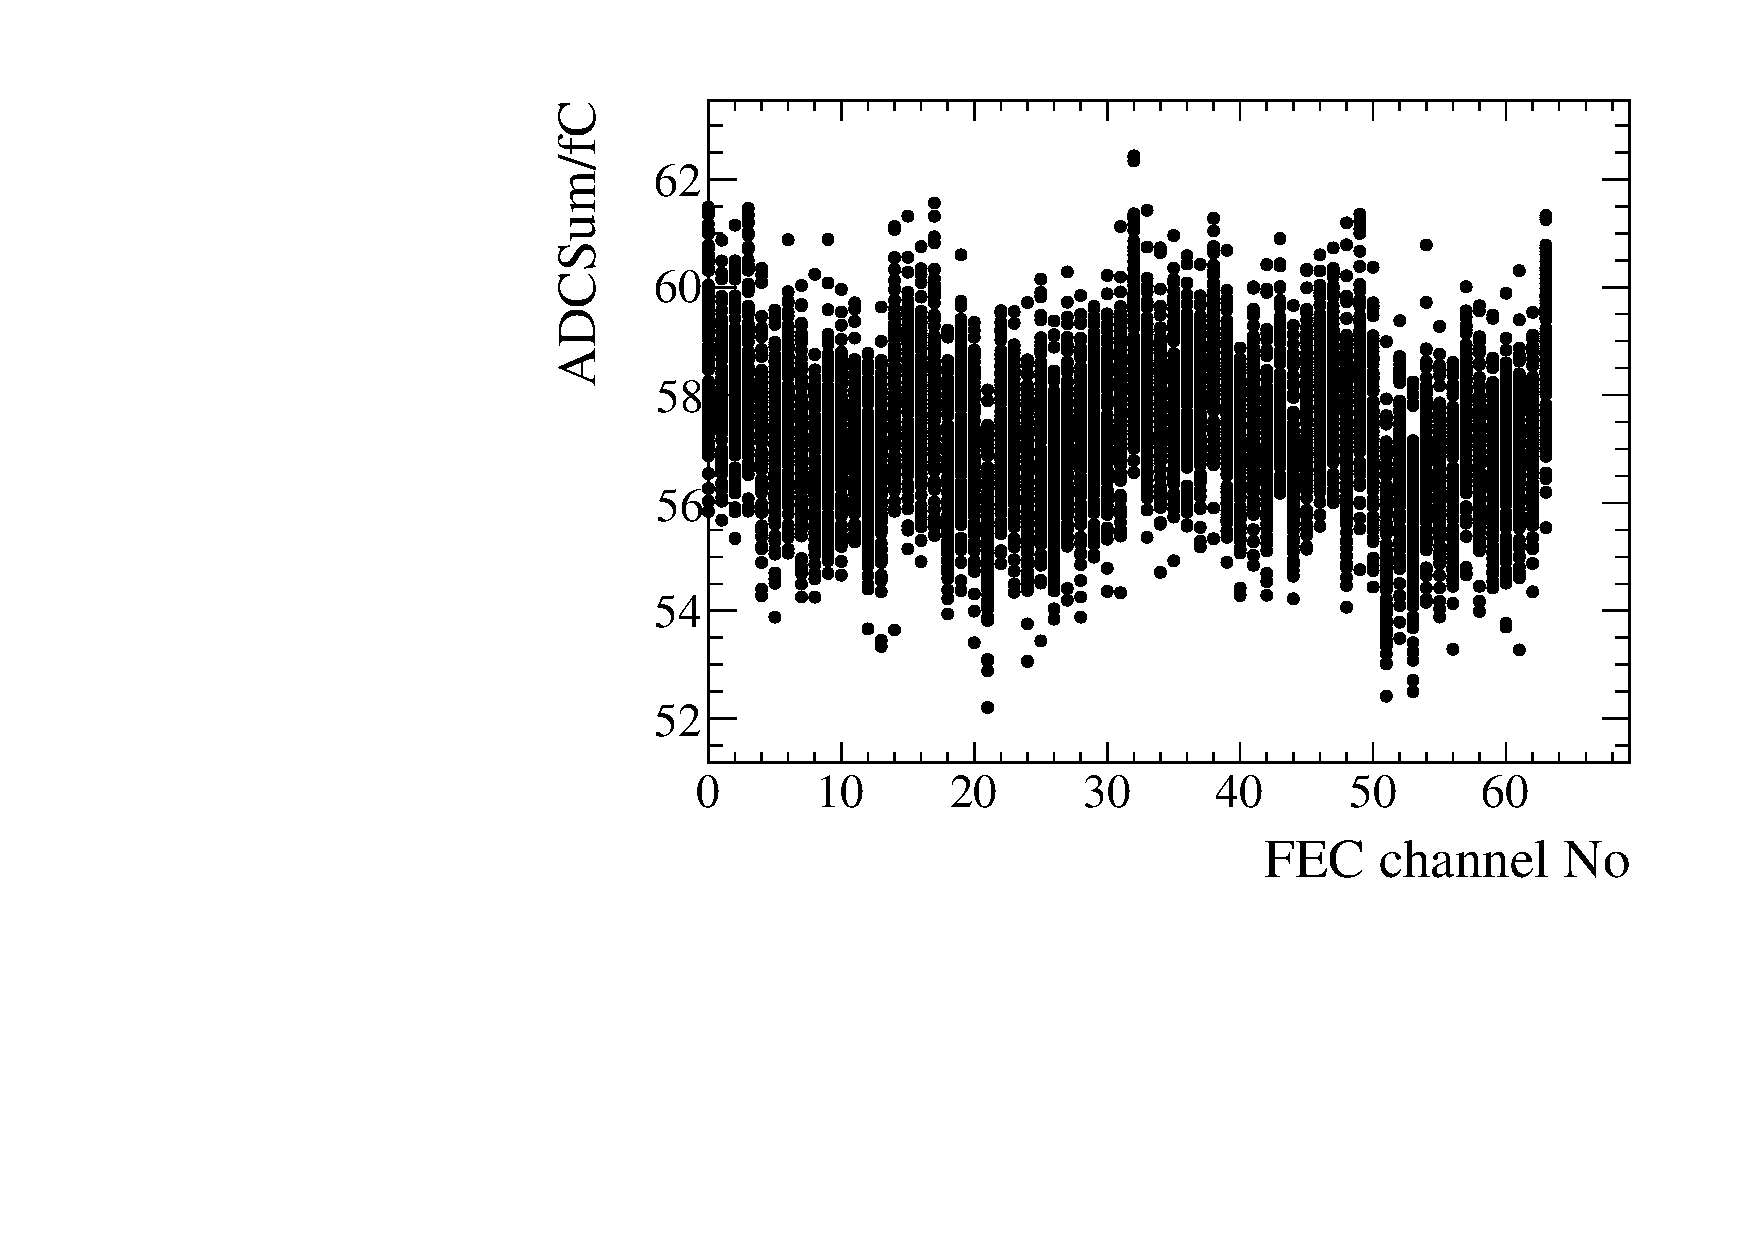
\includegraphics[width=0.45\textwidth]{dp-tpcelec-fec-calib-chnum}
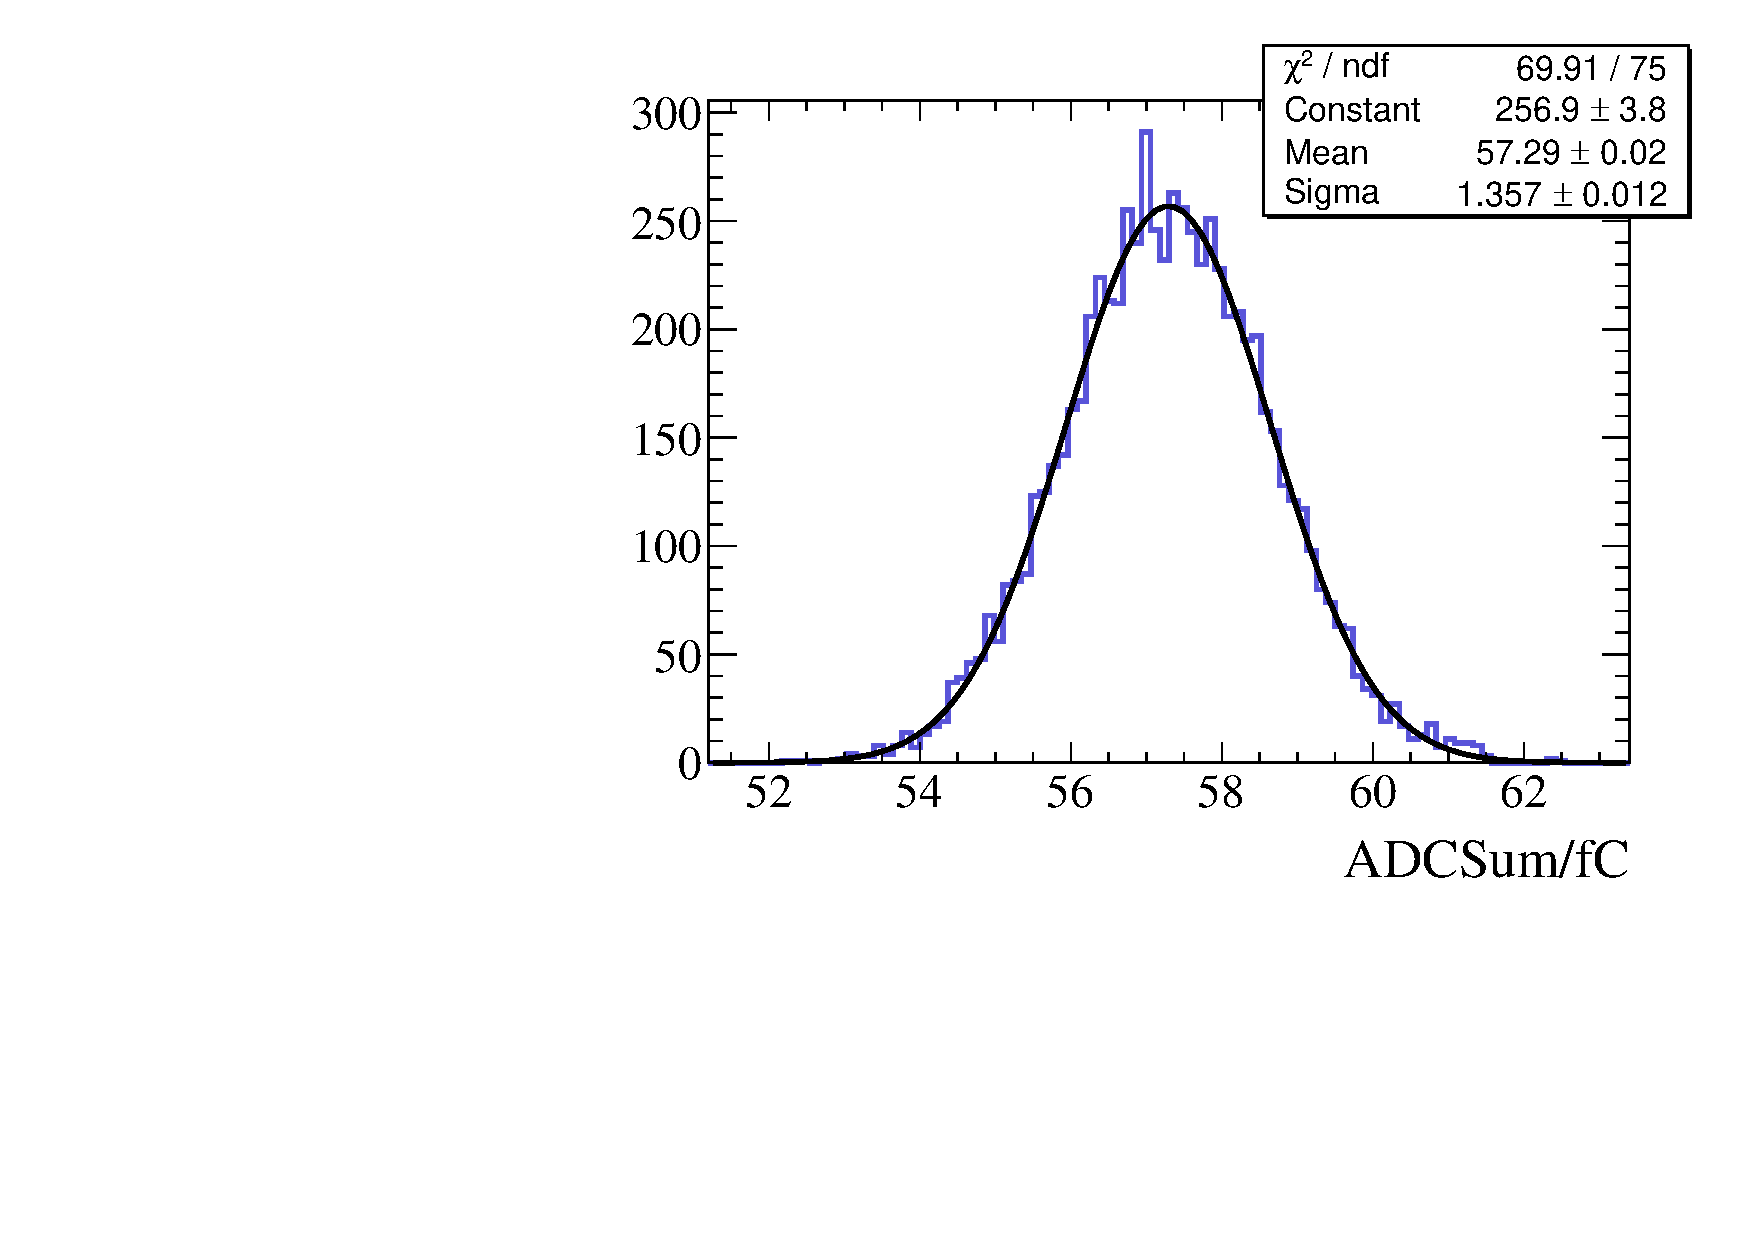
\includegraphics[width=0.45\textwidth]{dp-tpcelec-fec-calib-adcsum}
\end{dunefigure}

As an example, Figure~\ref{fig:dp-tpcelec-fec-calib} illustrates the channel-to-channel gain uniformity from the measurements performed with the \dword{fe} cards produced for \dword{pddp}. The figure on the %right 
left shows the gain (in units of pulse integral per unit of injected charge) as a function of channel number for all the cards tested, while that on the right shows the resultant distribution. The small sytematic variations in gain visible in the left-hand plot  arise from channel-to-channel variations in the injection card used for calibration of the \dword{fe} amplifiers. Overall the gain uniformity for all the channels is at the level of \SI{2}{\percent}.


%%%%%%%%%%%%%%%%%%%%%%%%%%%%%%%%%
\subsection{Signal Feedthrough Chimneys}
\label{ssec:dp-tpcelec-prod-sft}

A number of items must be manufactured to produce the \dwords{sftchimney}. These include 
\begin{itemize}
\item the PCB flanges for the warm and cold \fdth flange interfaces, 
\item the stainless steel pipe structure, 
\item the flanges containing the interfaces to the gas and liquid lines and slow control, 
\item the blades and railing, and 
\item the heat exchanger system. 
\end{itemize}
The flat cables that connect the \dword{fe} cards to the warm flange are commercially available products and part of the \dword{sftchimney} procurement process. 

The manufactured components are delivered to designated institutions participating in the \dual electronics consortium where teams verify signal continuity for both cold and warm flanges, then assemble the components into \dwords{sftchimney} and test for leaks. They also check blade insertion, and test flat cables.% , and then, once verified, 
After verification, they pack the assembled \dwords{sftchimney} and ship them to \dword{surf}. 

The commercial VHDCI signal cables (connecting the \dwords{amc} to the \dwords{sftchimney}) are procured and tested with the \dword{sftchimney} warm flanges.


%%%%%%%%%%%%%%%%%%%%%%%%%%%%%%%%%
\subsection{Timing System and $\mu$TCA}
\label{ssec:dp-tpcelec-prod-utca}

A \dword{utca} crate equipped with \dword{mch} and \dword{wrmch} will host the \dwords{amc} to be tested and calibrated. Triggering follows the same scheme as in \dword{pddp}, relying on the distribution of timestamped trigger packets over the \dword{wr} network to the \dwords{amc}. The triggers are generated by a high-precision pulse generator %synchronously 
sychronized with the calibration pulse signals sent to the analog or digital electronics. 

The timing system components,  the  \num{16} \dword{wr} switches and the \num{245} \dword{utca} crates containing the power modules, carrier hubs (\dword{mch}), and fan units, are commercially available. The manufacturer is responsible for the necessary \dword{qa} and \dword{qc}  of these components, requiring no further testing on the part of the \dual electronics consortium. Once the components are delivered to the designated institutions, they can be sent to \dword{surf} for installation. 



%%%%%%%%%%%%%%%%%%%%%%%%%%%%%%%%%
\subsection{Charge Readout Electronics}
\label{ssec:dp-tpcelec-prod-cro}

Production of the \dword{amc} cards for the charge readout and the \dword{wrmch} slave cards for synchronization is currently shared among four institutions (IPNL, KEK, NITKC, and IU). 
\fixme{these institutions do production, who does qa or qc tests?} The cards ordered and delivered to each institution are subjected to \dword{qc}  tests agreed upon by all participants. \fixme{prev pgraph said QA, I think it should be QC, so I changed it}

The \dword{qc} procedure for \dword{wrmch} cards nominally consists of 
\begin{itemize}
\item{checking the alignment of \dword{pps} signals between the \dword{wr} switch acting as the network grand master (Figure~\ref{fig:dp-tpcelec-qc-chain}) and each \dword{wrmch} slave node, and }
\item{performing data acquisition with functioning \dwords{amc} and verifying the quality of collected data.}
\end{itemize}

To calibrate the \dword{cro}  electronics, a dedicated calibration card %has been developed to 
injects  a known amount of charge into individual \dword{asic} channels via a precision capacitor to verify their functionality and calibrate the gain of the amplifiers. The channel selection is automatically performed via a multiplexer. To calibrate the \dword{adc} buffer of the \dword{cro} \dwords{amc}, we inject a known pulse into the input stage and measure the resulting pulse height after the digitization. 



The functionality of \dwords{amc} could be verified by performing acquisition of the pedestal data. In the case of \dword{pddp} production, this test allowed us to identify all the problems in the cards, almost all of which% . Almost all of them 
were a result of defective soldering that was not spotted by the automated \dword{qc} procedure of the manufacturer. 


%%%%%%%%%%%%%%%%%%%%%%%%%%%%%%%%%  
\subsection{Light Readout Electronics}
\label{ssec:dp-tpcelec-prod-lro}

Both \dword{lro} \dword{amc} cards are produced like the cards for \dword{pddp} because the number of cards produced and the channels to test are both small. The electronic components of the cards, which meet the required specifications, are purchased commercially. This part of the project will be managed by a qualified engineer working with a specialist in \dword{qa}.
\fixme{Need to clarify first sentence above}

The cards are delivered to designated consortium institutions. Upon delivery, teams conduct basic quality tests, including visual inspection and electrical testing, to ensure conformity of production. Another series of tests will ensure the cards' % function 
correct %ly 
functionality and will also evaluate their performance. Measurements include linearity measurements (DNL and INL) of each \dword{adc} channel and linearity of response of the \dword{asic}. The level of cross-talk on the \dword{asic} is also quantified. \fixme{what's DNL and INL?}

A dedicated single-channel set up, with a \dword{pmt} (Hamamatsu R5912-02-mod), and with the identical cabling and splitter as in the \dword{fd}, 
\fixme{the \dword{dpmod}?} 
can be used to characterize the expected noise level of each channel and the response to single \phel{}s, up to saturation. 
Several cards operate in each \dword{utca} crate with \dword{daq}. \fixme{last sentence not clear to me}

After shipment to \dword{surf} and on-site installation, a series of tests will be performed with a pulse generator to verify that the cards are in good working condition. Noise-level measurements are also included during integration.
